% simple.tex - A simple article to illustrate document structure.

% Arshad Ansari

\documentclass[12pt]{book}
\usepackage[T1]{fontenc}
\usepackage[utf8]{inputenc}
\usepackage{anyfontsize}
\usepackage{mathptmx}
\usepackage{graphicx}
\usepackage[margin=1in]{geometry}
\usepackage{mdwlist}
\usepackage{longtable}
\usepackage{mathtools}
\usepackage{float}
\graphicspath{ {figures/} }


\begin{document}

% Front Cover page
\thispagestyle{empty}

\begin{center}
	\fontsize{14}{30}\selectfont \textbf{A\\SPECIAL TOPIC SEMINAR\\ On}\\
  	\fontsize{20}{30}\selectfont \textbf{Text Classification Techniques}\\
  	\fontsize{14}{24}\selectfont Submitted in partial fulfillment of the requirement of Universirty of Mumbai\\For the Degree of\\
  	\fontsize{16}{30}\selectfont \textbf{Master of Engineering}\\
  	\fontsize{14}{30}\selectfont \textbf{Information Technology (AI and Robotics)} \\
  	by\\
  	\textbf{Mr. Mohammed Arshad Ansari}\\
  	\textbf{Registeration No: XYZ,}\\
  	Supervisor\\
  	\textbf{Prof. Sharvari Govilkar}\\
	\vspace{30mm}
	\begin{figure}[ht!]
	  \centering
	  
\includegraphics[width=30mm]{piit.png}
	\end{figure}
  	\fontsize{14}{20}\selectfont \textbf{DEPARTMENT OF INFORMATION TECHNOLOGY\\PILLAI'S INSTITUTE OF INFORMATION TECHNOLOGY,\\
	ENGINEERING, MEDIA STUDIES \& RESEARCH\\ NEW PANVEL - 410206\\UNIVERSITY OF MUMBAI\\Academic Year 2014-15}

\end{center}

% Certificate page
\begin{figure}[ht!]
    \centering
    
\includegraphics[width=30mm]{piit.png}
\end{figure}
\begin{center}
    \fontsize{14}{30}\selectfont \textbf{DEPARTMENT OF COMPUTER ENGINEERING\\PILLAI INSTITUTE OF INFORMATION TECHNOLOGY,\\ENGINEERING, MEDIA STUDIES \& RESEARCH\\ NEW PANVEL}\\
    \fontsize{22}{30}\selectfont \textbf{\underline{CERTIFICATE}}\\
    \fontsize{14}{30}\selectfont \textit{This is to certify that}\\
    \fontsize{14}{30}\selectfont \textbf{Mr. Mohammed Arshad Ansari}\\
    \fontsize{14}{30}\selectfont \textit{have satisfactorily completed the requirements of the Special Topic Seminar entitled}\\
    \fontsize{14}{30}\selectfont \textbf{On}\\
    \fontsize{20}{30}\selectfont \textbf{TEXT CLASSIFICATION TECHNIQUES}\\
    \fontsize{14}{30}\selectfont \textit{as prescribed by the \textbf{University of Mumbai}, under the guidance of \textbf{Prof. Sharvari Govilkar}}\\
    \vspace{20mm}
    \noindent --------------------------\hfill--------------------------\\
    \noindent Project Guide \hfill HOD\\
    \noindent\hfill \fontsize{14}{20}\selectfont Department of Information Technology\\
    \vspace{20mm}
    \noindent --------------------------\hfill--------------------------\\
    \noindent Internal Examiner\hfill External Examiner\\



\end{center}
	

% Acknowledgement page
\begin{center}

	\vspace{30mm}
    \fontsize{24}{60}\selectfont \textbf{Acknowledgement}\\
    \vspace{20mm}

		
	\fontsize{12}{20}\selectfont \raggedright{I am using this opportunity to express my gratitude to everyone who supported me throughout the course of my time in ME. I am thankful for their aspiring guidance, invaluably constructive criticism and friendy advice during the work. I am sincerely grateful to them for sharing their truthful and illuminating views on a number of issues related to the project.}\\
    \vspace{10mm}
	I express my warm thanks to our HOD, Mr Satish Verma for his support, consideration and guidance.
	Finally, a special thanks and humble appreciation of my project guide, Mrs. Sharvari Govilkar for making this happen. Her guidance, support and vision is what enabled this work and will enable what follows after this. \\
    \vspace{10mm}
	I would also like to thank all the people who provided me with the facilities being required and conductive conditions for my ME seminar.

    \vspace{60mm}
    \noindent\hfill \fontsize{14}{20}\selectfont -----------------------------\\
    \noindent\hfill \fontsize{14}{20}\selectfont Mohammed Arshad Ansari
\end{center}

\begin{center}
  \vspace{30mm}
  \fontsize{24}{60}\selectfont \textbf{Abstract}\\
  \vspace{20mm}

	\fontsize{12}{20}\selectfont \raggedright{The current work presents the current standard of text classification review for the purpose of selecting the best approach to create an intelligent way of classifying unstructured data in the ecommerce industry.
	Herein this work, we will look at the most accepted way of text classification in the industry to improve upon it and use for the work at hand in the Ensuant Inc's Toovia.com. }
	\vspace{10mm}
	There are two major approaches for text classfication using machine learning, each of which has a few techniques that were readily accepted in industry. They are supervised and unsupervised learning approaches and techniques such as Naive Bayes, Support Vector Machines, K-Nearest Neighbour, Expectation Minimization algorithms, etc. 
	\vspace{10mm}
	We will look into  each of these techinques in the work that follows and evaluate them based on the experiences shared by the authors of works that has been discussed and as a result, conclude upon the techniques that will be best suitable for the task at hand.

\end{center}

\tableofcontents


\addcontentsline{toc}{chapter}{i. List of Figures}
\listoffigures

\addcontentsline{toc}{chapter}{ii. List of Tables}
\listoftables

\clearpage

\pagenumbering{arabic}

\chapter{Introduction}

Text classification or Document classification is a problem in library science, information science and computer science. The task is to assign a document to one or more classes or categories. This may be done "manually" (or "intellectually") or algorithmically. The intellectual classification of documents has mostly been the province of library science, while the algorithmic classification of documents is used mainly in information science and computer science. The problems are overlapping, however, and there is therefore also interdisciplinary research on document classification.

The documents to be classified may be texts, images, music, etc. Each kind of document possesses its special classification problems. When not otherwise specified, text classification is implied.

Documents may be classified according to their subjects or according to other attributes (such as document type, author, printing year etc.). In the rest of this article only subject classification is considered. There are two main philosophies of subject classification of documents: The content based approach and the request based approach. \cite{wikipedia-textclassification}

\section{Types of classification}
Content based classification is classification in which the weight given to particular subjects in a document determines the class to which the document is assigned. It is, for example, a rule in much library classification that at least 20\% of the content of a book should be about the class to which the book is assigned.In automatic classification it could be the number of times given words appears in a document.

Request oriented classification (or -indexing) is classification in which the anticipated request from users is influencing how documents are being classified. The classifier asks himself: “Under which descriptors should this entity be found?” and “think of all the possible queries and decide for which ones the entity at hand is relevant” (Soergel, 1985, p. 230[2]).

Request oriented classification may be classification that is targeted towards a particular audience or user group. For example, a library or a database for feminist studies may classify/index documents differently when compared to a historical library. It is probably better, however, to understand request oriented classification as policy based classification: The classification is done according to some ideals and reflects the purpose of the library or database doing the classification. In this way it is not necessarily a kind of classification or indexing based on user studies. Only if empirical data about use or users are applied should request oriented classification be regarded as a user-based approach.

\textbf{Automatic document classification} tasks can be divided into three sorts: \\
\begin{itemize*}
  \item \textbf{\textit{Supervised document classification}}; where some external mechanism (such as human feedback) provides information on the correct classification for documents, \\
  \item \textbf{\textit{Unsupervised document classification}}; (also known as document clustering), where the classification must be done entirely without reference to external information, and \\
  \item \textbf{\textit{Semi-supervised document classification}}: where parts of the documents are labeled by the external mechanism.
\end{itemize*}


\section{Techniques for classification}


\begin{enumerate*}
  \item \textbf{\textit {Expectation maximization (EM)}}: The EM algorithm proceeds from the observation that the following is a way to solve these two sets of equations numerically. One can simply pick arbitrary values for one of the two sets of unknowns, use them to estimate the second set, then use these new values to find a better estimate of the first set, and then keep alternating between the two until the resulting values both converge to fixed points. It's not obvious that this will work at all, but in fact it can be proven that in this particular context it does, and that the derivative of the likelihood is (arbitrarily close to) zero at that point, which in turn means that the point is either a maximum or a saddle point.
  \item \textbf{\textit {Naive Bayes classifier}}: In simple terms, a naive Bayes classifier assumes that the value of a particular feature is unrelated to the presence or absence of any other feature, given the class variable. For example, a fruit may be considered to be an apple if it is red, round, and about 3" in diameter. A naive Bayes classifier considers each of these features to contribute independently to the probability that this fruit is an apple, regardless of the presence or absence of the other features.\\For some types of probability models, naive Bayes classifiers can be trained very efficiently in a supervised learning setting. In many practical applications, parameter estimation for naive Bayes models uses the method of maximum likelihood; in other words, one can work with the naive Bayes model without accepting Bayesian probability or using any Bayesian methods.
  \item \textbf{\textit {tf–idf}}:  is a numerical statistic that is intended to reflect how important a word is to a document in a collection or corpus.[1]:8 It is often used as a weighting factor in information retrieval and text mining. The tf-idf value increases proportionally to the number of times a word appears in the document, but is offset by the frequency of the word in the corpus, which helps to control for the fact that some words are generally more common than others.\\ Variations of the tf–idf weighting scheme are often used by search engines as a central tool in scoring and ranking a document's relevance given a user query. tf–idf can be successfully used for stop-words filtering in various subject fields including text summarization and classification.
  \item \textbf{\textit {Latent semantic indexing}}: is an indexing and retrieval method that uses a mathematical technique called singular value decomposition (SVD) to identify patterns in the relationships between the terms and concepts contained in an unstructured collection of text. LSI is based on the principle that words that are used in the same contexts tend to have similar meanings. A key feature of LSI is its ability to extract the conceptual content of a body of text by establishing associations between those terms that occur in similar contexts.
  \item \textbf{\textit {Support vector machines (SVM)}}: is  supervised learning models with associated learning algorithms that analyze data and recognize patterns, used for classification and regression analysis. Given a set of training examples, each marked as belonging to one of two categories, an SVM training algorithm builds a model that assigns new examples into one category or the other, making it a non-probabilistic binary linear classifier. An SVM model is a representation of the examples as points in space, mapped so that the examples of the separate categories are divided by a clear gap that is as wide as possible. New examples are then mapped into that same space and predicted to belong to a category based on which side of the gap they fall on.
  \item \textbf{\textit {Artificial neural network}}: are computational models inspired by an animal's central nervous systems (in particular the brain), and are used to estimate or approximate functions that can depend on a large number of inputs and are generally unknown. Artificial neural networks are generally presented as systems of interconnected "neurons" which can compute values from inputs, and are capable of learning thanks to their adaptive nature.
  \item \textbf{\textit {K-nearest neighbour algorithms}}:  is a non-parametric method used for classification and regression.[1] In both cases, the input consists of the k closest training examples in the feature space. The output depends on whether k-NN is used for classification or regression:
	\begin{itemize*}
	  \item In k-NN classification, the output is a class membership. An object is classified by a majority vote of its neighbors, with the object being assigned to the class most common among its k nearest neighbors (k is a positive integer, typically small). If k = 1, then the object is simply assigned to the class of that single nearest neighbor.
	  \item In k-NN regression, the output is the property value for the object. This value is the average of the values of its k nearest neighbors.
	\end{itemize*}
  \item \textbf{\textit {Decision trees such as ID3 or C4.5}}: uses a decision tree as a predictive model which maps observations about an item to conclusions about the item's target value. It is one of the predictive modelling approaches used in statistics, data mining and machine learning. More descriptive names for such tree models are classification trees or regression trees. In these tree structures, leaves represent class labels and branches represent conjunctions of features that lead to those class labels.
  \item \textbf{\textit {Concept Mining}}:  is an activity that results in the extraction of concepts from artifacts. Solutions to the task typically involve aspects of artificial intelligence and statistics, such as data mining and text mining.[1] Because artifacts are typically a loosely structured sequence of words and other symbols (rather than concepts), the problem is nontrivial, but it can provide powerful insights into the meaning, provenance and similarity of documents.
  \item \textbf{\textit {Multiple-instance learning}}: is a variation on supervised learning. Instead of receiving a set of instances which are individually labeled, the learner receives a set of labeled bags, each containing many instances. In the simple case of multiple-instance binary classification, a bag may be labeled negative if all the instances in it are negative. On the other hand, a bag is labeled positive if there is at least one instance in it which is positive. From a collection of labeled bags, the learner tries to either (i) induce a concept that will label individual instances correctly or (ii) learn how to label bags without inducing the concept.
  \item \textbf{\textit {Natural language processing approaches}}:  is a field of computer science, artificial intelligence, and linguistics concerned with the interactions between computers and human (natural) languages. As such, NLP is related to the area of human–computer interaction. Many challenges in NLP involve natural language understanding, that is, enabling computers to derive meaning from human or natural language input, and others involve natural language generation.
\end{enumerate*}

\section{Problem Domain}
Here the problem domain under consideration is an ecommerce platform that collects product information from the web and does the following tasks.
\begin{itemize*}
  \item Find similarity between products (at individual level) to group them together as same products and allow price differenciation.
  \item Find similarity between products at a macroscopic level to group them together as belonging to same category of products automatically.
  \item Find cross related products, to group them based on their function. E.g. Grouping similar pants and shirts together.
\end{itemize*}

Although, all the above mentioned aspects are a problem of different type, there is a need for three of them from the same business reason. Which is to  create an experience that does the thinking for the users on these sites. Therefore, the objective is to come to a concensus with the techniques, which  used individually or in hybrid way, to accomplish most of the above mentioned objectives. The scope of current report is to evaluate the techniques mentioned previously, their latest development and their suitability to the problem. Here we will not be exhaustively considering all the techniques, since some of them clearly do not fit the bill and are out of the scope of this report. For example, if we consider techniques such as Expectation maximization, Artificial neural network, Multiple instance learning, KNN, etc, 
then they are either highly supervised and/or unsupervised. Since the problem domain is of business importance we will be using tools available to us, and one such tool is the existance of just such categorization data that was done manually as well as the title being the best way to compare the product's complete similarity and the existence of product groups on the retailer's websites (which is the source of all data). These tools
provide us with data that is not complete and can only partially train the learning algorithms. Therefore, we would be mostly interested in semi supervised classification where part of the learning will be done via the existing labels and part of it will be done through some clustering mechanism to extend those labels. 


\chapter{Literature Survey}

In this work, research listed in following table was referred to understand the current scenario in the field of text classification.
The conclusions from the work will be referenced later in the report, where we will look into the different types of techniques involved.


\begin{longtable}[c]{ |p{3cm}|p{3cm}|p{3cm}|p{3cm}|  }
  \caption{Existing Papers on the topic \label{tab:existing_worexisting_work}}\\
  \hline
  Paper & Author & Approach & Result\\
  \hline
  \endhead

  A Machine Learning Approach for Automatic Text Categorization & Kurt Maly, Steven Zeil,  Mohammed Zubair, Naveen Ratkal& SVM is used to classify the Defence Technical Information Center documents in to their appropriate category& SVM out perform other techniques such as bayes and KNN classifiers as shown in this work\\ 
  \hline
  Automatic Text Classification: A Technical Review & Mita K. Dalal, Mukesh A. Zaveri & Multiple techniques are used for classification and evaluated in this work.& Stress must be given on feature selection, size and quality of training data to influence accuracy and correctness.\\ 
  \hline
  Online News Text Classification Using Neural Network and SVM& Raghvan Gachli & Techniques such as Backpropagation Algorithm and SVM are used for text classification in this work. & Credence is given to the mixed (hybrid) approach for classification.\\ 
  \hline
  Appyling Machine Learning to Product Categorization & Sushant Shankar and Irving Lin& Multiple techniques evaluated such as Naive Bayes, SVM and KNN. & Different data set yeild different results. Classification based on category set with ranking is given more suitablity in case of heirachy of categories\\ 
  \hline
  Building semantic kernels for Text Classification using Wikipedia& Pu Wang and Carlotta Domeniconi& Bag of Words approach is improved by applying the knowledge from wikipedia to the sematic kernals that will be used by the BOW technique for a more informed classification. & The overall bag of words based performance is enhanced due to more promity between synomyms, which are derived from the semantic kernals.\\ 
  \hline
  GoldenBullet: Automated Classification of Product Data in E-commerce & Y. Ding, M. Korotkiy, B. Omelayenko, V. Kartseva, V. Zykov, M. Klien, E. Schulten and D. Fensel & A system called GoldenBullet is explained and evaluation for the purpose of text classification. & It uses a hybrid approach of combining data mining and machine learning techniques. The yeild is somewhere between 70\% to 98\%\\
  \hline

\end{longtable}

\section{Review Literature}
Let's revisit the work of the above mentioned papers and see what they concluded in a little bit detailed fashion.
\subsection{Practicality of purpose}
In almost all the papers, there were mixed feelings between fast and not so accurate classifers versus the not so fast and accurate classifiers. Every paper suggested that if the speed is the key, then naive-bayes outperforms most of the techniques, 
with the exception of SVM. In may cases, where the learning is not adaptive, using the clustering algorithms for their accuracy is suggested. As can be seen from the different view points, the speed does become a very throttling factor, when it comes 
to the world wide web, where the solutions must be presented with lightening speed.

\subsection{Learning reusability verses the parallelization}
In some instances, where the learning is divided across multiple classifiers, due to the differences in the task under consideration, it becomes to reuse the learning from one classifier to another. It will enable the system to outperform any single classifier based system.
However, there is one obvious catch. It makes the system less parallel. Since there is sharing of learning, the classifiers need to communicate with one another, and hence, wait for one another to do the communication. This in some cases makes the classifers to behave in 
serial fashion, where one classifer feeds its learning to the other. However, for fast system, parallelizaton is a matter of real concern and therefore, some means needs to be agreed upon to do a trade off between the two necessities.

\subsection{Classification versus clustering}
There are instances where the clustering will be a good fit for solving the problem, where as, in come cases classifier will do just fine. The identification of this is a bit cumbersome. Usually, classification is supervised, whereas, clustering is unsupervised. So, it does seem
that one can be sure of where to apply what. But this assumption breaks down as soon as we consider the amount of data avaiable for supervised learning, which is accurate and the amount of data, that needs to be actaully classifed. To add to that, there is a great possibility of 
new data entering system, which was never considered by the supervised learning. This new data would skew the decision making in one direction or the other without having a valid reason behind it.

\subsection{Domain knowledge}
Many of the machine learning tasks can be made focussed by adding some existing domain knowledge to the mix. This helps in the correctly identifying the concept as per the domain requirement, which may change from ecommerce to defence. This is a very valid and necessary optimization
that must be inculcated in every system that is being designed to learn. This gives rise to the need of structured domain repository of concepts that would be placed there by manual work. For many problem domains like e-commmerce, there exists such repository of information and for some 
that data needs to be created. Evern in case of existing repository of domain knowledge, it must be customized to fit the actual problem that is being solved by the system under consideration.

\chapter{Other topics related to the seminar}

Before we embark onto the understanding of the text classification, it is time to see the big picture of where does the whole idea of text classification techniques fit. We will cover some major topic overview and then go on in to look at major techniques for classificiation in the later sections. 

\section{Text Mining}
Text mining\cite{wikipedia-textmining}, also referred to as text data mining, roughly equivalent to text analytics, refers to the process of deriving high-quality information from text. High-quality information is typically derived through the devising of patterns and trends through means such as statistical pattern learning. Text mining usually involves the process of structuring the input text (usually parsing, along with the addition of some derived linguistic features and the removal of others, and subsequent insertion into a database), deriving patterns within the structured data, and finally evaluation and interpretation of the output. 'High quality' in text mining usually refers to some combination of relevance, novelty, and interestingness. Typical text mining tasks include text categorization, text clustering, concept/entity extraction, production of granular taxonomies, sentiment analysis, document summarization, and entity relation modeling (i.e., learning relations between named entities).

Text analysis involves information retrieval, lexical analysis to study word frequency distributions, pattern recognition, tagging/annotation, information extraction, data mining techniques including link and association analysis, visualization, and predictive analytics. The overarching goal is, essentially, to turn text into data for analysis, via application of natural language processing (NLP) and analytical methods.

\section{Text analysis processes}
The process involves the steps for analysis purpose as show below\cite{wikipedia-textmining}:
\begin{itemize*}
  \item Information Retrieval or identification of a corpus is a preparatory step: collecting or identifying a set of textual materials, on the Web or held in a file system, database, or content management system, for analysis. 
  \item Although some text analytics systems apply exclusively advanced statistical methods, many others apply more extensive natural language processing, such as part of speech tagging, syntactic parsing, and other types of linguistic analysis
  \item Named entity recognition is the use of gazetteers or statistical techniques to identify named text features: people, organizations, place names, stock ticker symbols, certain abbreviations, and so on. Disambiguation — the use of contextual clues — may be required to decide where, for instance, "Ford" can refer to a former U.S. president, a vehicle manufacturer, a movie star, a river crossing, or some other entity.
  \item Recognition of Pattern Identified Entities: Features such as telephone numbers, e-mail addresses, quantities (with units) can be discerned via regular expression or other pattern matches.
  \item Coreference: identification of noun phrases and other terms that refer to the same object.
  \item Relationship, fact, and event Extraction: identification of associations among entities and other information in text
  \item Sentiment analysis involves discerning subjective (as opposed to factual) material and extracting various forms of attitudinal information: sentiment, opinion, mood, and emotion. Text analytics techniques are helpful in analyzing sentiment at the entity, concept, or topic level and in distinguishing opinion holder and opinion object.
  \item Quantitative text analysis is a set of techniques stemming from the social sciences where either a human judge or a computer extracts semantic or grammatical relationships between words in order to find out the meaning or stylistic patterns of, usually, a casual personal text for the purpose of psychological profiling etc.
\end{itemize*}

\section{Information retrieval}
Information retrieval\cite{wikipedia-inforet} is the activity of obtaining information resources relevant to an information need from a collection of information resources. Searches can be based on metadata or on full-text (or other content-based) indexing.

Automated information retrieval systems are used to reduce what has been called "information overload". Many universities and public libraries use IR systems to provide access to books, journals and other documents. Web search engines are the most visible IR applications.

\subsection{First dimension: mathematical basis}
\begin{itemize*}
  \item Set-theoretic models represent documents as sets of words or phrases. Similarities are usually derived from set-theoretic operations on those sets. 
  \item Algebraic models represent documents and queries usually as vectors, matrices, or tuples. The similarity of the query vector and document vector is represented as a scalar value.
  \item Probabilistic models treat the process of document retrieval as a probabilistic inference. Similarities are computed as probabilities that a document is relevant for a given query. Probabilistic theorems like the Bayes' theorem are often used in these models.
  \item Feature-based retrieval models view documents as vectors of values of feature functions (or just features) and seek the best way to combine these features into a single relevance score, typically by learning to rank methods. Feature functions are arbitrary functions of document and query, and as such can easily incorporate almost any other retrieval model as just a yet another feature.
\end{itemize*}

\subsection{Second dimension: properties of the model}
\begin{itemize*}
  \item Models without term-interdependencies treat different terms/words as independent. This fact is usually represented in vector space models by the orthogonality assumption of term vectors or in probabilistic models by an independency assumption for term variables.
  \item Models with immanent term interdependencies allow a representation of interdependencies between terms. However the degree of the interdependency between two terms is defined by the model itself. It is usually directly or indirectly derived (e.g. by dimensional reduction) from the co-occurrence of those terms in the whole set of documents.
  \item Models with transcendent term interdependencies allow a representation of interdependencies between terms, but they do not allege how the interdependency between two terms is defined. They relay an external source for the degree of interdependency between two terms. (For example a human or sophisticated algorithms.)
\end{itemize*}

\section{Natural language processing}
Natural language processing (NLP)\cite{wikipedia-nlp} is a field of computer science, artificial intelligence, and linguistics concerned with the interactions between computers and human (natural) languages. As such, NLP is related to the area of human–computer interaction. Many challenges in NLP involve natural language understanding, that is, enabling computers to derive meaning from human or natural language input, and others involve natural language generation.

The following is a list of some of the most commonly researched tasks in NLP. Note that some of these tasks have direct real-world applications, while others more commonly serve as sub-tasks that are used to aid in solving larger tasks. 
\subsection{Automatic Summarization}
Produce a readable summary of a chunk of text. Often used to provide summaries of text of a known type, such as articles in the financial section of a newspaper.

\subsection{Coreference resolution}
Given a sentence or larger chunk of text, determine which words ("mentions") refer to the same objects ("entities"). Anaphora resolution is a specific example of this task, and is specifically concerned with matching up pronouns with the nouns or names that they refer to. The more general task of coreference resolution also includes identifying so-called "bridging relationships" involving referring expressions. For example, in a sentence such as "He entered John's house through the front door", "the front door" is a referring expression and the bridging relationship to be identified is the fact that the door being referred to is the front door of John's house (rather than of some other structure that might also be referred to).
\subsection{Discourse analysis}
This rubric includes a number of related tasks. One task is identifying the discourse structure of connected text, i.e. the nature of the discourse relationships between sentences (e.g. elaboration, explanation, contrast). Another possible task is recognizing and classifying the speech acts in a chunk of text (e.g. yes-no question, content question, statement, assertion, etc.).
\subsection{Machine translation}
Automatically translate text from one human language to another. This is one of the most difficult problems, and is a member of a class of problems colloquially termed "AI-complete", i.e. requiring all of the different types of knowledge that humans possess (grammar, semantics, facts about the real world, etc.) in order to solve properly.
\subsection{Morphological segmentation}
Separate words into individual morphemes and identify the class of the morphemes. The difficulty of this task depends greatly on the complexity of the morphology (i.e. the structure of words) of the language being considered. English has fairly simple morphology, especially inflectional morphology, and thus it is often possible to ignore this task entirely and simply model all possible forms of a word (e.g. "open, opens, opened, opening") as separate words. In languages such as Turkish, however, such an approach is not possible, as each dictionary entry has thousands of possible word forms.
\subsection{Named entity recognition (NER)}
Given a stream of text, determine which items in the text map to proper names, such as people or places, and what the type of each such name is (e.g. person, location, organization). Note that, although capitalization can aid in recognizing named entities in languages such as English, this information cannot aid in determining the type of named entity, and in any case is often inaccurate or insufficient. For example, the first word of a sentence is also capitalized, and named entities often span several words, only some of which are capitalized. Furthermore, many other languages in non-Western scripts (e.g. Chinese or Arabic) do not have any capitalization at all, and even languages with capitalization may not consistently use it to distinguish names. For example, German capitalizes all nouns, regardless of whether they refer to names, and French and Spanish do not capitalize names that serve as adjectives.
\subsection{Part-of-speech tagging}
Given a sentence, determine the part of speech for each word. Many words, especially common ones, can serve as multiple parts of speech. For example, "book" can be a noun ("the book on the table") or verb ("to book a flight"); "set" can be a noun, verb or adjective; and "out" can be any of at least five different parts of speech. Some languages have more such ambiguity than others. Languages with little inflectional morphology, such as English are particularly prone to such ambiguity. Chinese is prone to such ambiguity because it is a tonal language during verbalization. Such inflection is not readily conveyed via the entities employed within the orthography to convey intended meaning.
\subsection{Sentiment analysis}
Extract subjective information usually from a set of documents, often using online reviews to determine "polarity" about specific objects. It is especially useful for identifying trends of public opinion in the social media, for the purpose of marketing.
\subsection{Topic segmentation and recognition}
Given a chunk of text, separate it into segments each of which is devoted to a topic, and identify the topic of the segment.
\subsection{Word segmentation}
Separate a chunk of continuous text into separate words. For a language like English, this is fairly trivial, since words are usually separated by spaces. However, some written languages like Chinese, Japanese and Thai do not mark word boundaries in such a fashion, and in those languages text segmentation is a significant task requiring knowledge of the vocabulary and morphology of words in the language.
\subsection{Word sense disambiguation}
Many words have more than one meaning; we have to select the meaning which makes the most sense in context. For this problem, we are typically given a list of words and associated word senses, e.g. from a dictionary or from an online resource such as WordNet.

\vspace{2cm}
From the next chapter onwards we will look at each of the techniques covered as part of this report, one by one and in depth.

%\begin{figure}
%\centering
%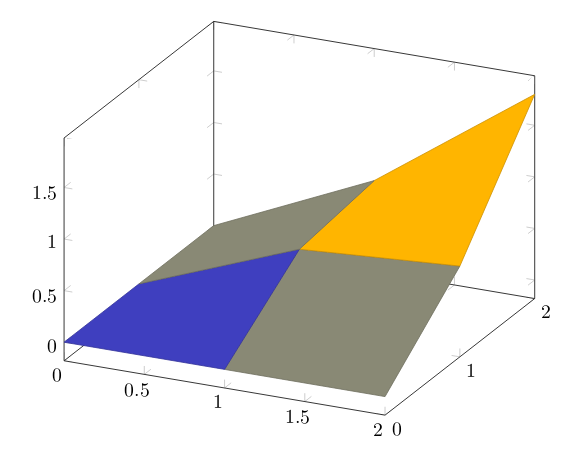
\includegraphics[width=8cm]{Pgfplot3d3}
%\caption{Three dimensional graph}
%\label{fig:figure1}
%\end{figure}


\chapter{Classification Techniques}

To understand classification in the text based domain it is essential to first come to terms with the problem statement that will be referred going forward, in order to validate the correctness of system under consideration. These definitions
may or may not be accurate for the given give problem domain for which the system is being built, therefore, there is a need for a generic statement to be made and validation to be performed against. 

\section{Definition of Problem}
The general text categorization task can be formally defined as the task of approx- imating an unknown category assignment function F : D x C -> {0, 1}, where D is the set of all possible documents and C is the set of predefined categories. The value of F(d, c) is 1 if the document d belongs to the category c and 0 otherwise. The approximating function M : D x C -> {0, 1} is called a classifier, and the task is to build a classifier that produces results as “close” as possible to the true category assignment function F.

\section{Document Representation}
The common classifiers and learning algorithms cannot directly process the text doc- uments in their original form. Therefore, during a preprocessing step, the documents are converted into a more manageable representation. Typically, the documents are represented by feature vectors. A feature is simply an entity without internal struc- ture – a dimension in the feature space. A document is represented as a vector in this space – a sequence of features and their weights.

\subsection{Feature Selection}

The number of different words is large even in relatively small documents such as short news articles or paper abstracts. The number of different words in big docu- ment collections can be huge. The dimension of the bag-of-words feature space for a big collection can reach hundreds of thousands; moreover, the document represen- tation vectors, although sparse, may still have hundreds and thousands of nonzero components.
Most of those words are irrelevant to the categorization task and can be dropped with no harm to the classifier performance and may even result in improvement owing to noise reduction. The preprocessing step that removes the irrelevant words is called feature selection. Most TC systems at least remove the stop words – the function words and in general the common words of the language that usually do not contribute to the semantics of the documents and have no real added value. Many systems, however, perform a much more aggressive filtering, removing 90 to 99 percent of all features.

In order to perform the filtering, a measure of the relevance of each feature needs to be defined. Probably the simplest such measure is the document frequency DocFreq(w). Experimental evidence suggests that using only the top 10 percent of the most frequent words does not reduce the performance of classifiers. This seems to contradict the well-known “law” of IR, according to which the terms with low-to-medium document frequency are the most informative. There is no contra- diction, however, because the large majority of all words have a very low document frequency, and the top 10 percent do contain all low-to-medium frequency words.

There are two techniques for doing feature selection as shown under.

\subsubsection{Information Gain}
The information gain method measures the number of bits of information obtained for the prediction of categories by knowing the presence or absence in a document of the feature f. The probabilities are computed as ratios of frequencies in the training data. 


$$IG(w) = \sum_{c \in C \bigcup \bar{C}} \sum_{f \in \{w, \bar{w}\}} P(f, c) \frac{P(c | f)}{P(c)}$$

\subsubsection{CHI Square Method}
 measures the maximal strength of dependence between the feature and the categories. Experiments show that both measures (and several other measures) can reduce the dimensionality by a factor of 100 without loss of categorization quality – or even with a small improvement.
 $$ x^2_{max}= max_{c \in C} \frac{\|Tr\| . (P(f, c) . P(\bar{f}, \bar{c}) - P(f, \bar{c}) . P(\bar{f}, c))^2}{P(f) . P(\bar{f}) . P(c) . P(\bar{c})} $$

\subsection{Dimensionality Reduction by Feature Extraction}
Another way of reducing the number of dimensions is to create a new, much smaller set of synthetic features from the original feature set. In effect, this amounts to creat- ing a transformation from the original feature space to another space of much lower dimension. The rationale for using synthetic features rather than naturally occur- ring words (as the simpler feature filtering method does) is that, owing to polysemy, homonymy, and synonymy, the words may not be the optimal features. By transform- ing the set of features it may be possible to create document representations that do not suffer from the problems inherent in those properties of natural language.
Term clustering addresses the problem of synonymy by grouping together words with a high degree of semantic relatedness. These word groups are then used as features instead of individual words. Experiments conducted by several groups of researchers showed a potential in this technique only when the background infor- mation about categories was used for clustering (Baker and McCallum 1998; Slonim and Tishby 2001). With unsupervised clustering, the results are inferior (Lewis 1992a, 1992b; Li and Jain 1998).
A more systematic approach is latent semantic indexing (LSI). The details of this method are described in Chapter V. For the TC problem, the performance of the LSI also improves if the categories information is used. Several LSI representations, one for each category, outperform a single global LSI representation. The experiments also show that LSI usually performs better than the chi-square filtering scheme.

\section{Machine Learning for Text Categorization}

In the ML approach, the classifier is built automatically by learning the properties of categories from a set of preclassified training documents. In the ML terminology, the learning process is an instance of supervised learning because the process is guided by applying the known true category assignment function on the training set.

\subsection{Naive Bayes Classifier\cite{wikipedia-naive}}

A naive Bayes classifier assumes that the value of a particular feature is unrelated to the presence or absence of any other feature, given the class variable. For example, a fruit may be considered to be an apple if it is red, round, and about 3" in diameter. A naive Bayes classifier considers each of these features to contribute independently to the probability that this fruit is an apple, regardless of the presence or absence of the other features.

For some types of probability models, naive Bayes classifiers can be trained very efficiently in a supervised learning setting. In many practical applications, parameter estimation for naive Bayes models uses the method of maximum likelihood; in other words, one can work with the naive Bayes model without accepting Bayesian probability or using any Bayesian methods.

Despite their naive design and apparently oversimplified assumptions, naive Bayes classifiers have worked quite well in many complex real-world situations. In 2004, an analysis of the Bayesian classification problem showed that there are sound theoretical reasons for the apparently implausible efficacy of naive Bayes classifiers.[5] Still, a comprehensive comparison with other classification algorithms in 2006 showed that Bayes classification is outperformed by other approaches, such as boosted trees or random forests.[6]

An advantage of naive Bayes is that it only requires a small amount of training data to estimate the parameters (means and variances of the variables) necessary for classification. Because independent variables are assumed, only the variances of the variables for each class need to be determined and not the entire covariance matrix.

\begin{figure}[H]
\centering
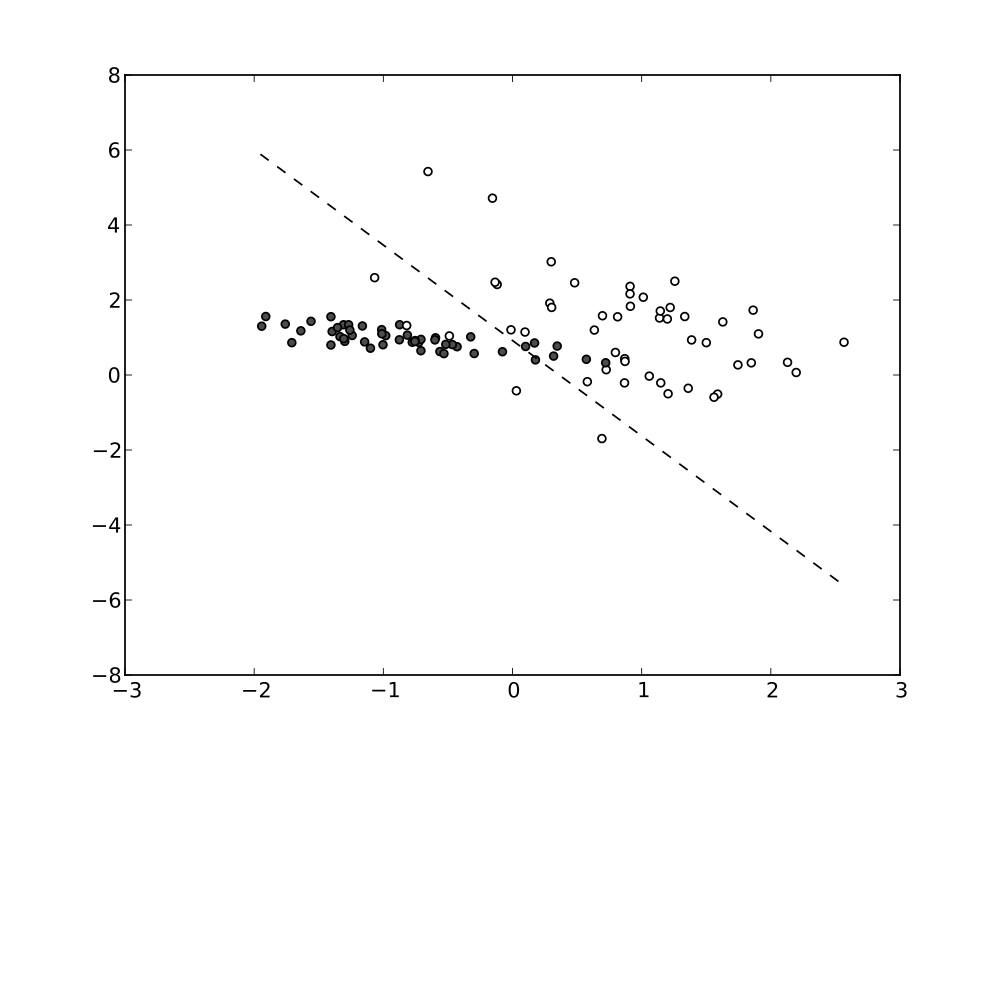
\includegraphics[width=8cm]{Linear-svm-scatterplot.png}
\caption{Naive Bayes Visualization\cite{wikipedia-naive}}
\label{fig:figure1}
\end{figure}

\subsubsection{Probabilistic model}
Abstractly, the probability model for a classifier is a conditional model over a dependent class variable $C$ with a small number of outcomes or classes, conditional on several feature variables $F_1$ through $F_n$. The problem is that if the number of features n is large or if a feature can take on a large number of values, then basing such a model on probability tables is infeasible. We therefore reformulate the model to make it more tractable.

$$ p(C|F_1\cdots F_2) $$

Using Bayes' theorem, this can be written as:

$$ p(C \vert F_1,\dots,F_n) = \frac{p(C) \ p(F_1,\dots,F_n\vert C)}{p(F_1,\dots,F_n)}. \,$$

In plain English, using Bayesian Probability terminology, the above equation can be written as

$$\mbox{posterior} = \frac{\mbox{prior} \times \mbox{likelihood}}{\mbox{evidence}}. \,$$

In practice, there is interest only in the numerator of that fraction, because the denominator does not depend on C and the values of the features $F_i$ are given, so that the denominator is effectively constant. The numerator is equivalent to the joint probability model

$$ p(C, F_1, \dots, F_n)\, $$
which can be rewritten as follows, using the chain rule for repeated applications of the definition of conditional probability:

\begin{align}
p(C, F_1, \dots, F_n) & = p(C) \ p(F_1,\dots,F_n\vert C) \\
                      & = p(C) \ p(F_1\vert C) \ p(F_2,\dots,F_n\vert C, F_1) \\
                      & = p(C) \ p(F_1\vert C) \ p(F_2\vert C, F_1) \ p(F_3,\dots,F_n\vert C, F_1, F_2) \\
                      & = p(C) \ p(F_1\vert C) \ p(F_2\vert C, F_1) \ \dots p(F_n\vert C, F_1, F_2, F_3,\dots,F_{n-1}) 
\end{align}
Now the "naive" conditional independence assumptions come into play: assume that each feature $F_i$ is conditionally independent of every other feature $F_j$ for $j\neq i$, given the category C. This means that

$$ p(F_i \vert C, F_j) = p(F_i \vert C)\,, $$
$$ p(F_i \vert C, F_j,F_k) = p(F_i \vert C)\,, $$
$$ p(F_i \vert C, F_j,F_k,F_l) = p(F_i \vert C)\,, $$
and so on, for  $i\ne j,k,l$. Thus, the joint model can be expressed as

This means that under the above independence assumptions, the conditional distribution over the class variable C is:
$$ p(C \vert F_1,\dots,F_n) = \frac{1}{Z}  p(C) \prod_{i=1}^n p(F_i \vert C)$$
where the evidence $Z = p(F_1, \dots, F_n)$ is a scaling factor dependent only on $F_1,\dots,F_n$, that is, a constant if the values of the feature variables are known.


\subsubsection{Example}

\textbf{Sex classification}
Problem: classify whether a given person is a male or a female based on the measured features. The features include height, weight, and foot size.

\begin{longtable}[c]{ |p{3cm}|p{3cm}|p{3cm}|p{3cm}|  }
  \caption{Example sex classification using naive bayes\label{tab:sex_classification_naive_bayes}}\\
  \hline
  sex & height (feet) & weight (lbs) & foot size(inches)\\
  \hline
  \endhead
  male & 6 & 180 & 12\\
  \hline
  male & 5.92 (5'11") & 190 & 11\\
  \hline
  male & 5.58 (5'7") & 170 & 12\\
  \hline
  male & 5.92 & (5'11") & 165 & 10\\
  \hline
  female & 5 & 100 & 6\\
  \hline
  female & 5.5 (5'6") & 150 & 8\\
  \hline
  female & 5.42 (5'5") & 130 & 7\\
  \hline
  female & 5.75 (5'9") & 150 & 9\\
  \hline
\end{longtable}

The classifier created from the training set using a Gaussian distribution assumption would be (given variances are sample variances):

\begin{longtable}[c]{ |p{2cm}|p{2cm}|p{2cm}|p{2cm}|p{2cm}|p{2cm}|p{2cm}|  }
  \caption{Example sex classification using naive bayes result \label{tab:sex_classification_naive_bayes_res}}\\
  \hline
  sex & mean (height) & variance (height) & mean (weight) & variance (weight) & mean (foot size) & variance (foot size)\\
  \hline
  \endhead
  male & 5.85 & 3.5033e-02 & 176.25 & 1.2292e+02 & 11.25 & 9.1667e-01\\
  \hline
  female & 5.41 & 9.7225e-02 & 132.5 & 5.5833e+02 & 7.5 & 1.6667e+00\\
  \hline
\end{longtable}
 
%\begin{align}
%p(C \vert F_1, \dots, F_n) & \varpropto p(C, F_1, \dots, F_n) \\
%                           & \varpropto p(C) \ p(F_1\vert C) \ p(F_2\vert C) \ p(F_3\vert C) \ \cdots \\
                           %& \varpropto p(C) \prod_{i=1}^n p(F_i \vert C)\,.
%\end{align}

\subsection{Support Vector Machine}
A support vector machine constructs a hyperplane or set of hyperplanes in a high- or infinite-dimensional space, which can 
be used for classification, regression, or other tasks. Intuitively, a good separation is achieved 
by the hyperplane that has the largest distance to the nearest training data point of any class (so-called functional margin), 
since in general the larger the margin the lower the generalization error of the classifier.

Whereas the original problem may be stated in a finite dimensional space, it often happens that the sets to discriminate are not linearly 
separable in that space. For this reason, it was proposed that the original finite-dimensional space be mapped into a much higher-dimensional 
space, presumably making the separation easier in that space. To keep the computational load reasonable, the mappings used by SVM schemes 
are designed to ensure that dot products may be computed easily in terms of the variables in the original space, by defining them in terms of 
a kernel function k(x,y) selected to suit the problem.[2] The hyperplanes in the higher-dimensional space are defined as the set of points whose dot 
product with a vector in that space is constant. The vectors defining the hyperplanes can be chosen to be linear combinations with parameters $\alpha_i$ 
of images of feature vectors that occur in the data base. With this choice of a hyperplane, the points x in the feature space that are mapped into the hyperplane are defined by the relation: 
$\textstyle\sum_i \alpha_i k(x_i,x) = \mathrm{constant}$. Note that if k(x,y) becomes small as y grows further away from x, each term in the sum 
measures the degree of closeness of the test point x to the corresponding data base point $x_i$. In this way, the sum of kernels above can be used to measure the relative
nearness of each test point to the data points originating in one or the other of the sets to be discriminated. Note the fact that the set of points x mapped into any hyperplane 
can be quite convoluted as a result, allowing much more complex discrimination between sets which are not convex at all in the original space.

Given some training data $\mathcal{D}$, a set of n points of the form

$$\mathcal{D} = \left\{ (\mathbf{x}_i, y_i) | \mathbf{x}_i \in \mathbf{R}^p,\, y_i \in \{-1,1\}\right\}_{i=1}^n$$

where the $y_i$ is either 1 or -1, indicating the class to which the point $\mathbf{x}_i$  belongs. Each  $\mathbf{x}_i$  is a p-dimensional real vector. 
We want to find the maximum-margin hyperplane that divides the points having $y_i=1$ from those having $y_i=-1$. Any hyperplane can be written as the set of points $\mathbf{x}$ satisfying

$$ \mathbf{w}\cdot\mathbf{x} - b=0,\, $$

where $\cdot$ denotes the dot product and ${\mathbf{w}}$ the (not necessarily normalized) normal vector to the hyperplane. The parameter $\tfrac{b}{\|\mathbf{w}\|}$ determines the offset of the 
hyperplane from the origin along the normal vector ${\mathbf{w}}$.

If the training data are linearly separable, we can select two hyperplanes in a way that they separate the data and there are no points between them, and then try to maximize their distance. 
The region bounded by them is called "the margin". These hyperplanes can be described by the equations

$$\mathbf{w}\cdot\mathbf{x} - b=1\,$$
and

$$\mathbf{w}\cdot\mathbf{x} - b=-1.\,$$
By using geometry, we find the distance between these two hyperplanes is $\tfrac{2}{\|\mathbf{w}\|}$, so we want to minimize $\|\mathbf{w}\|$. As we also have to prevent data points from falling into the margin, we add the following constraint: for each i either

$\mathbf{w}\cdot\mathbf{x}_i - b \ge 1\qquad\text{ for }\mathbf{x}_i $ of the first class
or

$\mathbf{w}\cdot\mathbf{x}_i - b \le -1\qquad\text{ for }\mathbf{x}_i $  of the second.
This can be rewritten as:

$$y_i(\mathbf{w}\cdot\mathbf{x}_i - b) \ge 1, \quad \text{ for all } 1 \le i \le n.\qquad\qquad(1) $$
We can put this together to get the optimization problem:

Minimize (in ${\mathbf{w},b}$)

$$\|\mathbf{w}\|$$
subject to (for any i = 1, \dots, n)

$$y_i(\mathbf{w}\cdot\mathbf{x_i} - b) \ge 1. \, $$

\begin{figure}[H]
\centering
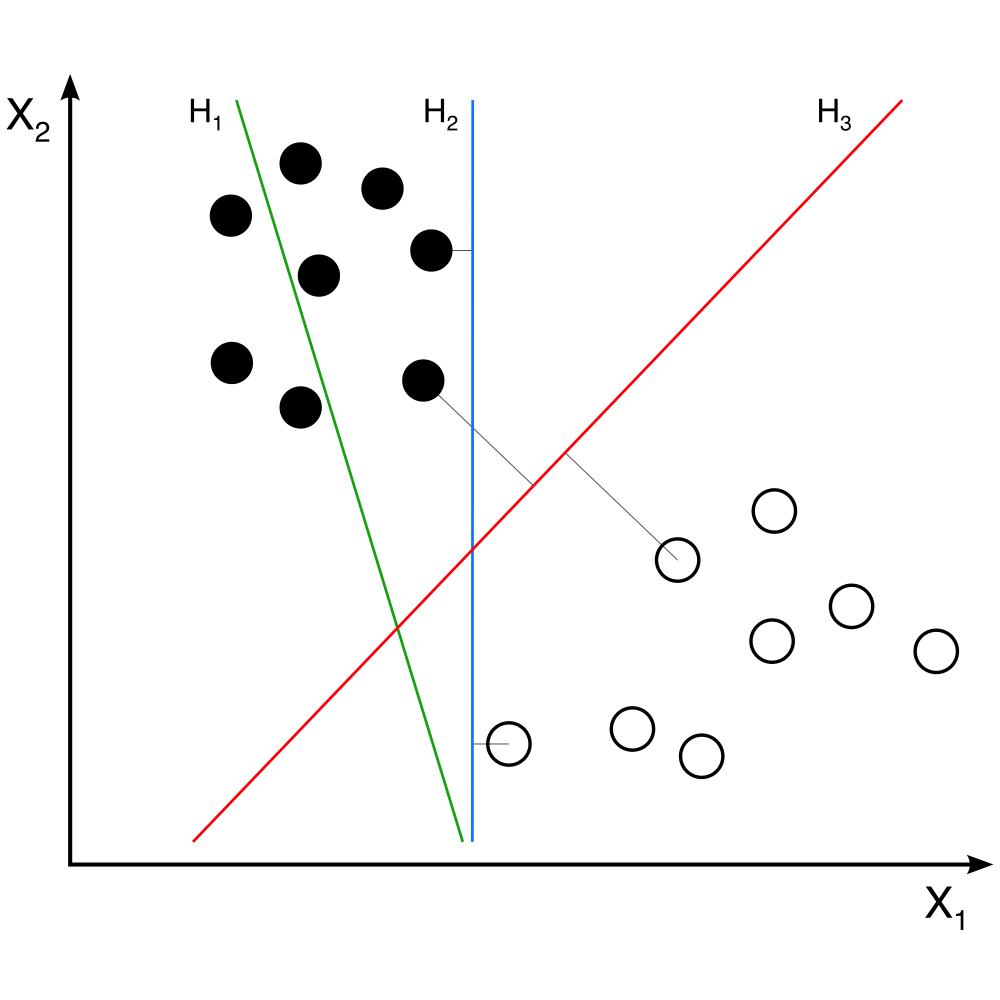
\includegraphics[width=8cm]{Svm2.png}
\caption{Support Vector Machine \cite{wikipedia-svm}}
\label{fig:figure2}
\end{figure}



\subsection{K Nearest Neighbour}
k-NN is a type of instance-based learning, or lazy learning, where the function is only approximated locally and all computation is deferred until classification. The k-NN algorithm is among the simplest of all machine learning algorithms.

Both for classification and regression, it can be useful to weight the contributions of the neighbors, so that the nearer neighbors contribute more to the average than the more distant ones. For example, a common weighting scheme consists in giving each neighbor a weight of 1/d, where d is the distance to the neighbor.[2]

The neighbors are taken from a set of objects for which the class (for k-NN classification) or the object property value (for k-NN regression) is known. This can be thought of as the training set for the algorithm, though no explicit training step is required.

A shortcoming of the k-NN algorithm is that it is sensitive to the local structure of the data.

\begin{figure}[H]
\centering
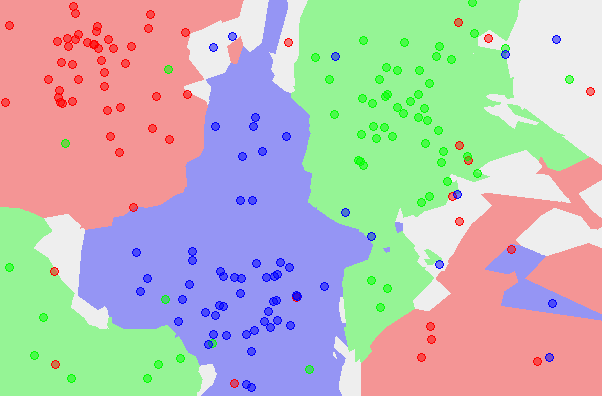
\includegraphics[width=8cm]{Map5NN.png}
\caption{K-Nearest Neighbors\cite{wikipedia-knn}}
\label{fig:figure4}
\end{figure}



\subsubsection{Algorithm}
The training examples are vectors in a multidimensional feature space, each with a class label. The training phase of the algorithm consists only of storing the feature vectors and class labels of the training samples.

In the classification phase, k is a user-defined constant, and an unlabeled vector (a query or test point) is classified by assigning the label which is most frequent among the k training samples nearest to that query point.

A commonly used distance metric for continuous variables is Euclidean distance. For discrete variables, such as for text classification, another metric can be used, such as the overlap metric (or Hamming distance). In the context of gene expression microarray data, for example, k-NN has also been employed with correlation coefficients such as Pearson and Spearman[3]. Often, the classification accuracy of k-NN can be improved significantly if the distance metric is learned with specialized algorithms such as Large Margin Nearest Neighbor or Neighbourhood components analysis.

A drawback of the basic "majority voting" classification occurs when the class distribution is skewed. That is, examples of a more frequent class tend to dominate the prediction of the new example, because they tend to be common among the k nearest neighbors due to their large number.[4] One way to overcome this problem is to weight the classification, taking into account the distance from the test point to each of its k nearest neighbors. The class (or value, in regression problems) of each of the k nearest points is multiplied by a weight proportional to the inverse of the distance from that point to the test point. Another way to overcome skew is by abstraction in data representation. For example in a self-organizing map (SOM), each node is a representative (a center) of a cluster of similar points, regardless of their density in the original training data. K-NN can then be applied to the SOM.

\subsubsection{Properties}
k-NN is a special case of a variable-bandwidth, kernel density "balloon" estimator with a uniform kernel.[8] [9]

The naive version of the algorithm is easy to implement by computing the distances from the test example to all stored examples, but it is computationally intensive for large training sets. Using an appropriate nearest neighbor search algorithm makes k-NN computationally tractable even for large data sets. Many nearest neighbor search algorithms have been proposed over the years; these generally seek to reduce the number of distance evaluations actually performed.

k-NN has some strong consistency results. As the amount of data approaches infinity, the algorithm is guaranteed to yield an error rate no worse than twice the Bayes error rate (the minimum achievable error rate given the distribution of the data).[10] k-NN is guaranteed to approach the Bayes error rate for some value of k (where k increases as a function of the number of data points). Various improvements to k-NN are possible by using proximity graphs.

\subsubsection{k-NN regression}
In k-NN regression, the k-NN algorithm is used for estimating continuous variables. One such algorithm uses a weighted average of the k nearest neighbors, weighted by the inverse of their distance. This algorithm works as follows:

\begin{itemize*}
  \item Compute the Euclidean or Mahalanobis distance from the query example to the labeled examples.
  \item Order the labeled examples by increasing distance.
  \item Find a heuristically optimal number k of nearest neighbors, based on RMSE. This is done using cross validation.
  \item Calculate an inverse distance weighted average with the k-nearest multivariate neighbors.
\end{itemize*}

\subsection{Expectation–maximization algorithm EM}
The EM algorithm is used to find the maximum likelihood parameters of a statistical model in cases where the equations cannot be solved directly. Typically these models involve latent variables 
in addition to unknown parameters and known data observations. That is, either there are missing values among the data, or the model can be formulated more simply by assuming the existence of 
additional unobserved data points. For example, a mixture model can be described more simply by assuming that each observed data point has a corresponding unobserved data point, or latent variable, 
specifying the mixture component that each data point belongs to.

Finding a maximum likelihood solution typically requires taking the derivatives of the likelihood function with respect to all the unknown values — viz. the parameters and the latent variables — 
and simultaneously solving the resulting equations. In statistical models with latent variables, this usually is not possible. Instead, the result is typically a set of interlocking equations in 
which the solution to the parameters requires the values of the latent variables and vice-versa, but substituting one set of equations into the other produces an unsolvable equation.

The EM algorithm proceeds from the observation that the following is a way to solve these two sets of equations numerically. One can simply pick arbitrary values for one of the two sets of unknowns, 
use them to estimate the second set, then use these new values to find a better estimate of the first set, and then keep alternating between the two until the resulting values both converge to fixed 
points. It's not obvious that this will work at all, but in fact it can be proven that in this particular context it does, and that the derivative of the likelihood is (arbitrarily close to) zero at 
that point, which in turn means that the point is either a maximum or a saddle point.[citation needed] In general there may be multiple maxima, and there is no guarantee that the global maximum will 
be found. Some likelihoods also have singularities in them, i.e. nonsensical maxima. For example, one of the "solutions" that may be found by EM in a mixture model involves setting one of the 
components to have zero variance and the mean parameter for the same component to be equal to one of the data points.

\subsubsection{Details}
Given a statistical model consisting of a set $\mathbf{X}$ of observed data, a set of unobserved latent data or missing values $\mathbf{Z}$, and a vector of unknown parameters $\boldsymbol\theta$, 
along with a likelihood function $L(\boldsymbol\theta; \mathbf{X}, \mathbf{Z}) = p(\mathbf{X}, \mathbf{Z}|\boldsymbol\theta)$, the maximum likelihood estimate (MLE) of the unknown parameters is 
determined by the marginal likelihood of the observed data

$L(\boldsymbol\theta; \mathbf{X}) = p(\mathbf{X}|\boldsymbol\theta) = \sum_{\mathbf{Z}} p(\mathbf{X},\mathbf{Z}|\boldsymbol\theta)$ 
However, this quantity is often intractable (e.g. if $\mathbf{Z}$ is a sequence of events, so that the number of values grows exponentially with the sequence length, making the exact calculation of 
the sum extremely difficult).

The EM algorithm seeks to find the MLE of the marginal likelihood by iteratively applying the following two steps:

Expectation step (E step): \\
Calculate the expected value of the log likelihood function, with respect to the conditional distribution of $\mathbf{Z}$ given $\mathbf{X}$ under the current estimate of the parameters \\
$$\boldsymbol\theta^{(t)}: Q(\boldsymbol\theta|\boldsymbol\theta^{(t)}) = \operatorname{E}_{\mathbf{Z}|\mathbf{X},\boldsymbol\theta^{(t)}}\left[ \log L (\boldsymbol\theta;\mathbf{X},\mathbf{Z})  \right] \,$$ \\
Maximization step (M step): Find the parameter that maximizes this quantity:\\
$$\boldsymbol\theta^{(t+1)} = \underset{\boldsymbol\theta}{\operatorname{arg\,max}} \ Q(\boldsymbol\theta|\boldsymbol\theta^{(t)}) \,$$\\

\subsubsection{Example}

This is a recipe to learn EM with a practical and (in my opinion) very intuitive 'Coin-Toss' example as shown in figure \cite{blog-em}.
\begin{figure}[H]
\centering
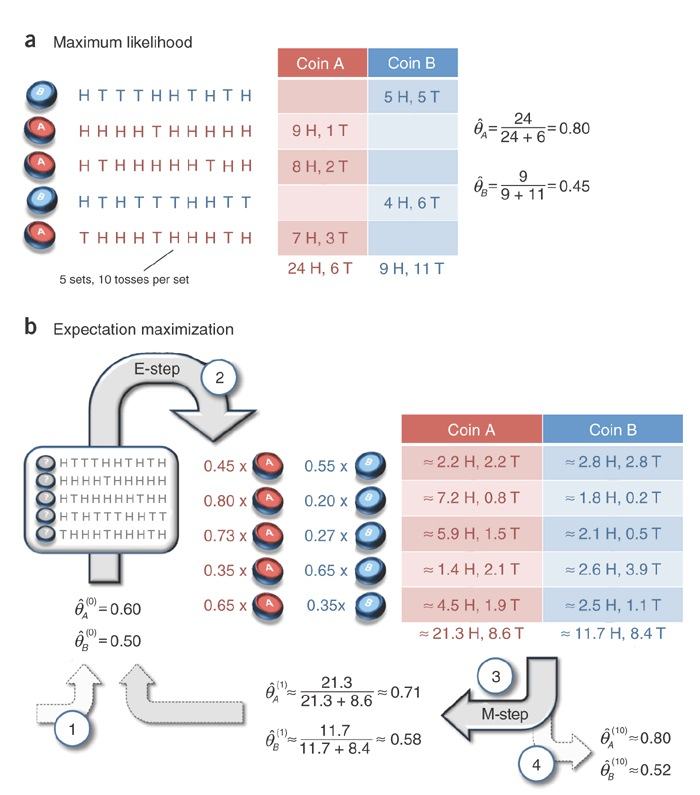
\includegraphics[width=8cm]{em.jpg}
\caption{EM Example\cite{blog-em}}
\label{fig:figure5}
\end{figure}

\subsection{Hybrid Approach}
Although the hybrid approach depends highly on the type of task at hand, here the hybrid is being mentioned only as a promise as it will be delivered only after the implementation of this system will be designed. It can be said, though, that the 
clustering and classification can both be used semi independently or cooperatively to achieve multiple goals in a given system. It is topic that will be further investigation as the problem domain becomes more clear in time and will become essential 
part of the implementation that will be done in the coming sememster.


\chapter{Applications}

\section{Applications in general}
Here we will look at two types of applications for our proposed work. One is outcome of its generacity and another is due to the specific focus of the objectives for this work. When we talk about general applications, following are the most obvious ones and
have been prevalently the raison-de-etre for this research.
\begin{itemize*}
  \item \textbf{Spam Filtering} a process which tries to discern E-mail spam messages from legitimate emails
  \item \textbf{Email Routing} sending an email sent to a general address to a specific address or mailbox depending on topic
  \item \textbf{Language Identification} automatically determining the language of a text
  \item \textbf{genre classification} automatically determining the genre of a text (also the objective of this work)
  \item \textbf{readability assessment} automatically determining the degree of readability of a text, either to find suitable materials for different age groups or reader types or as part of a larger text simplification system 
  \item \textbf{sentiment analysis} determining the attitude of a speaker or a writer with respect to some topic or the overall contextual polarity of a document.
  \item \textbf{Article triage} selecting articles that are relevant for manual literature curation, for example as is being done as the first step to generate manually curated annotation databases in biology.
\end{itemize*}

\section{Application in Ecommerce}

The proposed work is relevant for many ecommerce site and especially in the company to which the author belongs. Toovia.com is an upcoming startup that envisions to be a portal for all the lifestyle products to be 
bought, reviewed and marketed from a single platform. Most of the products there are coming from different ecommerce sites. Each of these sites have similar/same products that must be identified as one with their discount differences maintained.
Not just that, it is also necessary to map the product from one section of the incoming product to the appropriate section of the host site and some times the categories used are not part of the same vocabulary.

\subsection{Identification of same products across retailers}
The idea is to use the classification/clustering methodology to find the similarity score between the products and hence mark them as same if the same product is coming from different retailers. This will enable the company to identify variety of
discounts and price differences and hence, leverage them to the benefit of the consumer or buyer. When products from different retailers come and are the same, it takes more storage space, show duplicates on the site and therefore are candiate for 
merging into a single product.

\subsection{Categorization to a common taxonomy}
When the retailers create their categories of products or taxonomies for their products, they do so based on their own worldview and niche. Which is why a sports site may have a deeper category for its products, which may not be generally needed by
other non - sports oriented site, which does sell the sports products. This lack of straight mapping between the categories is the prime motivator for which this task is being undertaken by the company, of which the author is the team lead. The 
completion of this task will free up lot of developers from doing the mapping of these categories manually and focus their time on coding instead of managing taxonomies. Also, in author's experience, most of the bugs we face in this kind of situation 
is when manual error causes a different product to be shown in different category. This work aims to bring down the number of such bugs to almost negligible amount.

\subsection{Filtering process for search enhancements}
Machine learning is the best way to find hidden models available inside the data, at the same time it makes sense out of unstructured data, such as text documents. This has one more added advantage which we will talk about here. It is really difficult 
to create or identify right kind of facets/parameters for enhancing the search in ecommerce where product data base is huge and is highly varient. In such cases, the idea of clustering really helps by returning the whole cluster if the search matches one
product from the given cluster. It enables the system to have more accurate search results and also to be able to recomment a similar of associated products. This increases the overall experience of the customer on an ecommerce site. The user's interaction
with the system can also be mapped to the type of products and reviews he/she views. This interaction will allow further classification of data as per the user's preference. This can also allow reduction in the types of products that is shown to the user,
especially when we know he is not really that interested in those kind of products.

\chapter{Conclusions}

Here are some general conclusions derived from this work..

\section{Question based}
\subsection{How large is your training set?}
If your training set is small, high bias/low variance classifiers (e.g., Naive Bayes) have an advantage over low bias/high variance classifiers (e.g., kNN or logistic regression), since the latter will overfit. But low bias/high variance classifiers start to win out as your training set grows (they have lower asymptotic error), since high bias classifiers aren't powerful enough to provide accurate models. 
You can also think of this as a generative model vs. discriminative model distinction.

\subsection{Advantages of some particular algorithms}
\subsubsection{Advantages of Naive Bayes} Super simple, you're just doing a bunch of counts. If the NB conditional independence assumption actually holds, a Naive Bayes classifier will converge quicker than discriminative models like logistic regression, so you need less training data. And even if the NB assumption doesn't hold, a NB classifier still often performs surprisingly well in practice. A good bet if you want to do some kind of semi-supervised learning, or want something embarrassingly simple that performs pretty well.

\subsubsection{Advantages of Logistic Regression} Lots of ways to regularize your model, and you don't have to worry as much about your features being correlated, like you do in Naive Bayes. You also have a nice probabilistic interpretation, unlike decision trees or SVMs, and you can easily update your model to take in new data (using an online gradient descent method), again unlike decision trees or SVMs. Use it if you want a probabilistic framework (e.g., to easily adjust classification thresholds, to say when you're unsure, or to get confidence intervals) or if you expect to receive more training data in the future that you want to be able to quickly incorporate into your model.

\subsubsection{Advantages of Decision Trees} Easy to interpret and explain (for some people -- I'm not sure I fall into this camp). Non-parametric, so you don't have to worry about outliers or whether the data is linearly separable (e.g., decision trees easily take care of cases where you have class A at the low end of some feature x, class B in the mid-range of feature x, and A again at the high end). Their main disadvantage is that they easily overfit, but that's where ensemble methods like random forests (or boosted trees) come in. Plus, random forests are often the winner for lots of problems in classification (usually slightly ahead of SVMs, I believe), they're fast and scalable, and you don't have to worry about tuning a bunch of parameters like you do with SVMs, so they seem to be quite popular these days.

\subsubsection{Advantages of SVMs} High accuracy, nice theoretical guarantees regarding overfitting, and with an appropriate kernel they can work well even if you're data isn't linearly separable in the base feature space. Especially popular in text classification problems where very high-dimensional spaces are the norm. Memory-intensive and kind of annoying to run and tune, though, so I think random forests are starting to steal the crown.

\section{Combined Approach}
The belief of the author of this work is to combine multiple techniques to gain multiple benefits. Use clustering to find similarity between products, and create a thesaurus of the incoming category information, consequently enabling the developers to use machine learning to map the disparate taxonomies to the host site taxonomy.

It can be achieved as under.
\subsubsection{Clustering for similarity score}
Use of clustering algorithms will give similarity score across products, which in turn will give the ability to find same products as duplicates as well as create a mapping between incoming product taxonomies and existing taxonomy.

\subsubsection{Classification for high performance}
Once the clustering is complete, it will give the mapping information, which will be used to train the classifier and this classifier will be used directly in realtime when actually performing the import of products from the retailer website.

Recall, though, that better data often beats better algorithms, and designing good features goes a long way. And if you have a huge dataset, your choice of classification algorithm might not really matter so much in terms of classification performance (so choose your algorithm based on speed or ease of use instead).
And if you really care about accuracy, you should definitely try a bunch of different classifiers and select the best one by cross-validation. Or, to take a lesson from the Netflix Prize and Middle Earth, just use an ensemble method to choose them all!

\begin{thebibliography}{12}
	\bibitem{wikipedia-textclassification}
	  Text Classification, Wikipedia,
	  \emph {http://en.wikipedia.org/wiki/Document\_classification}.
	\bibitem{paper-atctechreview}
	  Automatic Text Classification,
	  Internation Journal of Computer Applications (0975 - 8888)
	  Volume 28 - No. 2, August 2011
	\bibitem{paper-ann-svm}
	  Online News Text Classification Using Neural Network and SVM,
	  Raghvan Gachli, International Journal of Latest Scientific Research and Technology 1(2), July - 2014, pp. 122-128, ISSN: 2348-9464
	\bibitem{paper-product-cat}
	  Applying Machine Learning to Product Categorization,
	  Sushant Shankar and Irving Lin,
	  Department of Computer Science, Standford University.
	\bibitem{paper-semantic-kernels}
	  Building Semantic Kernels for Text Classification using Wikipedia,
	  Pu Wang and Carlotta Domeniconi,
	  Department of Computer Science, George Mason University.
	\bibitem{paper-goldenbullet}
	  GoldenBullet: Automated Classification of Product Data in E-Commerce,
	  Y. Ding, M. Korotkiy, B. Omelayenko, V. Kartseva, V. Zykov, M. Klien, E. Schulten and D. Fensel.
	  Vrije Universiteit Amsterdam, De Boelelaan 1081a, 1081 HV Amsterdam, NL.
	\bibitem{wikipedia-textmining}
	  Text Minign, Wikipedia,\\
	  \emph {http://en.wikipedia.org/wiki/Text\_mining}.
	\bibitem{wikipedia-inforet}
	  Information Retrieval, Wikipedia,\\
	  \emph {http://en.wikipedia.org/wiki/Information\_retrieval}.
	\bibitem{wikipedia-nlp}
	  Natural Language Processing, Wikipedia,\\
	  \emph {http://en.wikipedia.org/wiki/Natural\_language\_processing}.
	\bibitem{wikipedia-naive}
	  Naive Bayes Algorithm, Wikipedia,\\
	  \emph {http://en.wikipedia.org/wiki/Naive\_Bayes\_classifier}.
	\bibitem{wikipedia-svm}
	  Support Vector Machine, Wikipedia,\\
	  \emph {http://en.wikipedia.org/wiki/Support\_vector\_machine}.
	\bibitem{wikipedia-knn}
	  K Nearest Neighbors, Wikipedia,\\
	  \emph {http://en.wikipedia.org/wiki/K-nearest\_neighbors\_algorithm}.
	\bibitem{wikipedia-em}
	  Expectation Maximization, Wikipedia,\\
	  \emph {http://en.wikipedia.org/wiki/Expectation\%E2\%80\%93maximization\_algorithm}.
	\bibitem{blog-em}
	  Numerical example to understand Expectation-Maximization, StackExchange.com\\
	  \emph {http://stats.stackexchange.com/questions/72774/numerical-example-to-understand-expectation-maximization}.



\end{thebibliography} %Must end the environment


\end{document}  %End of document.
